\documentclass[a4paper, 12pt]{article}
\usepackage[utf8]{inputenc}
\usepackage{graphicx}
\usepackage{amsmath}
\usepackage{hyperref}
\usepackage{caption}
\usepackage{subcaption}
\usepackage{float}

\title{Simulación Multiagente \\ Gestión de Proyectos.}
\author{Roger Fuentes Rodr\'iguez \\ Kevin Manzano Rodr\'iguez \\ Jackson Vera Pineda}
\date{\today}

\begin{document}

\maketitle

\section{Introducción}
En este informe presentamos el desarrollo de una simulación multiagente basada en una arquitectura BDI (Beliefs, Desires, Intentions). El enfoque de esta simulación está en la interacción entre dos tipos de agentes: el \textbf{Project Manager (PM)} y los \textbf{Trabajadores}, enfocándonos en la capacidad de gestión y dirección del primero. Además, se modeló un entorno dinámico donde los agentes interactúan con proyectos, definidos mediante una ontología que relaciona las tareas, recursos, riesgos y oportunidades del mismo.

El objetivo principal fue simular la gestión de proyectos en un entorno de trabajo utilizando técnicas de inteligencia artificial, incluyendo \textbf{algoritmos genéticos}, \textbf{lógica difusa}, \textbf{aprendizaje reforzado}, y \textbf{LLMs} lo que permitió optimizar la asignación de tareas y la resolución de problemas en tiempo real.

\section{Arquitectura BDI}
El modelo BDI permite a los agentes razonar sobre sus creencias, deseos e intenciones, adaptándose a situaciones dinámicas y cambiantes en el contexto del proyecto. Los agentes toman decisiones basadas en su percepción del entorno y en los objetivos que se les asignan.

\subsection{Beliefs (Creencias)}
El agente Project Manager mantienen una representación interna de su entorno, que incluye información sobre el estado del proyecto, los recursos disponibles, los riesgos identificados, el progreso de las tareas y de los agentes con los que interactúa, en este caso los trabajadores. En sus creencias posee un conjunto de reglas que modifican sus deseos, y un subconjunto de dichas reglas serán las reglas activas, las que se aplicarán cada vez que el agente actúa. Dichas reglas no son un conjunto estático, ya que existen algunas que pueden crear nuevas reglas y activarlas o eliminar reglas ya existentes. Para la creación de reglas el agente toma ciertas condiciones en que se encuentra el medio, y se apoya en un LLM, pasándole dichas condiciones y el conjunto de deseos, esperando como respuesta un subconjunto de condiciones que implicarían la activación de un subconjunto de deseos, elegimos esta forma para mantener cierto sentido sobre las reglas. De esta forma creamos un conjunto variado de reglas para diferentes situaciones, permitiendo al agente adaptar su comportamiento según el estado del medio en que se encuentra y cambiando las prioridades del proyecto consigo. Las reglas tienen un peso, el cual será modificado a medida que se aplique y se observe su efectividad. 
El Project Manager no va a crear reglas continuamente, de ser así el conjunto de las mismas sería exponencial además de repetir reglas o tener poca variedad entre ellas, para decidir cuándo crearlas nos hemos apoyado en la lógica difusa. Nuestro agente se apoya en una función que caracterizará el medio en el que se encuentra, considerando el progreso del proyecto. Usamos funciones de pertenencia como Nivel de motivación, recompenzas obtenidas, tiempo transcurrido, etc ; pasando dichos parámetros obtenemos sus valores fusificados, aplicamos las reglas definidas y obtenemos un valor categórico de como va el proyecto(mal, normal, bien). Esto nos permite evaluar la efectividad de las reglas que se han estado aplicando hasta ese momento y nos indica la necesidad de generar nuevas.

Los agentes Trabajadores mantienen una representación interna de las tareas que tienen asignadas, el progreso en las mismas, la motivación del equipo, algunas relaciones con otros agentes y ciertos parámetros que caracterízan al agente, como cuan trabajador es o su capacidad de resolución de problemas. Al igual que el Project Manager también posee un conjunto de reglas en sus creencias que modificarán sus deseos.

\subsection{Desires (Deseos)}
Los deseos reflejan los objetivos tanto a corto como a largo plazo que el agente intenta alcanzar, como completar un número máximo de tareas, evitar problemas o minimizar los recursos utilizados. Se incluyen deseos básicos de los seres humanos como descansar, mantener cierto nivel de motivación o cooperar con otros agentes. Los deseos de los trabajadores son más personales, sin embargo los del Project Manager contemplan además los deseos con el proyecto y con el equipo en general.

\subsection{Intentions (Intenciones)}
Las intenciones son los planes que el agente decide llevar a cabo en función de sus deseos, sus creencias y sus percepciones; como asignar recursos a tareas específicas o escalar problemas al Project Manager. Están más cerca de lo que el agente puede hacer para cumplir esos deseos, aquí se maneja cómo el agente actuará ante deseos contradictorios como descansar y trabajar, digamos que aquí se define el orden de prioridad de los deseos y la acción que devolverá el agente.

\section{Algoritmo Genético para la Planificación de Tareas}
El \textbf{Project Manager} utiliza un algoritmo genético para encontrar la mejor permutación posible de las tareas del proyecto debido a que no hay garant\'ia en que exista una permutación en la que se cumplan todas las restricciones de las tareas. A continuación, describimos el proceso:

\subsection{Población y Generación de Individuos}
Se parte de una población inicial compuesta por permutaciones siguiendo una heurística \textbf{greedy} para garantizar como m\'inimo las dependencias entre las tareas. Cada individuo de la población representa una permutación de las tareas del proyecto. Obtenemos un orden topol\'ogico de las tareas, con una modificaci\'on en el momento de la elecci\'on de los nodos con indegree $0$, este se elige de manera aleatoria. Luego de establecido el orden, los nodos quedan divididos en niveles, sobre estos niveles se realizan cambios de manera aleatoria.

\subsection{Selección y Cruzamiento}
Para seleccionar los individuos que pasarán a la siguiente generación, implementamos un método de \textbf{selección por torneo}, teniendo en cuenta un factor de elitismo que puede variar. Este método selecciona a los individuos más aptos para cruzarse y producir nuevos descendientes. Posteriormente, los individuos se cruzan y las mutaciones se incorporan como nuevos individuos, lo que permite introducir variabilidad en la población. Para el cruce de dos permutaciones dadas, $p_1, p_2$, se elige un punto de corte aleatorio de la primera permutación luego se van agregando nodos en el orden de la segunda permutaci\'on que no incumplan con las dependencias, y cuando termina este proceso puede darse el caso de que falten elementos por colocar, por lo tanto se rellenan con elementos en el orden de la primera permutación pues ya en esta se ha garantizado que se cumplen las dependencias.

\subsection{Mutación}
La mutación en este contexto implica la creación de nuevas permutaciones de tareas, introduciendo cambios aleatorios menores en los individuos seleccionados para diversificar la búsqueda del óptimo global. Se prioriza la diversidad de la dificultad entre las tareas sucesivas, lo que permite un mejor balance en la distribución de las tareas. Dada una permutación $p$, se elige un nodo aleatorio, luego se "empuja" este nodo en los niveles del orden topl\'ologico, de manera que se garantice que no se rompan las dependencias (los nodos que dependen de el también se empujaran).

\subsection{Función de Optimización}
Definimos dos funciones de optimización para el algoritmo. Una función pondera las restricciones cumplidas e incumplidas de las tareas en la permutación, como su posición respecto a su fecha mínima de comienzo y su fecha de terminación máxima o sus dependencias hacia otras tareas. Esta función devuelve un valor numérico y resultó más efectiva.
La otra función utilizada para evaluar la calidad de cada permutación de tareas incluye varios factores que pueden ajustarse mediante reglas de \textbf{lógica difusa}, esta función nos brinda una mayor flexibilidad a la hora de darle prioridades a ciertos parámetros sobre otros, ya que al crear reglas nuevas no tendríamos que modificar el código cada vez que cambie el objetivo del proyecto o crear varias funciones muy parecidas, el equipo propone crear un conjunto de conjuntos de reglas donde cada conjunto tribute a priorizar alguno de los parámetros a evaluar en las tareas; por ejemplo otorgar mayor peso al número de tareas posibles a completar frente a la calidad de las mismas.

Se incorporaron penalizaciones basadas en el incumplimiento de dependencias entre tareas, el exceso de tareas de dificultad similar y las tareas que exceden su \textit{deadline}. Además, se aplican bonificaciones por mantener una variedad de dificultades consecutivas y completar las tareas de alta prioridad a tiempo.

\section{Interacción entre Agentes}
Una vez que el \textbf{Project Manager} obtiene la mejor permutación de tareas, comienza la interacción con los \textbf{Trabajadores}. El PM asigna tareas a los trabajadores, supervisa su desarrollo y ajusta las estrategias en función del progreso.

\subsection{Asignación de Tareas Basada en Habilidades}
La asignación de tareas se basa en las habilidades de los trabajadores y la dificultad de las tareas. El PM utiliza una heurística que busca minimizar la diferencia entre la dificultad de la tarea y la capacidad de resolución de problemas del trabajador, garantizando una asignación eficiente.

\subsection{Generación de Hitos}
El PM genera \textbf{hitos} basados en proyecciones del avance del proyecto. Estos hitos no son estáticos, sino que se generan dinámicamente según la situación actual del proyecto. Para esto, el agente evalúa el estado del proyecto utilizando \textbf{lógica difusa}, lo que le permite proyectar los hitos de manera flexible, ajustándose a cambios en el entorno. Dependiendo del estado del equipo (motivación, productividad, disponibilidad de recursos), los hitos pueden ser conservadores, normales o entusiastas. El cumplimiento de los mismos también influye sobre la percepción del agente del estado del proyecto.

\section{Modelado del Proyecto con Ontologías}
Para representar los proyectos y su estructura, utilizamos una \textbf{ontología} que incluye los siguientes componentes:
\begin{itemize}
    \item \textbf{Recursos}: Elementos que el proyecto requiere para completarse, relacionados con las tareas.
    \item \textbf{Riesgos}: Posibles problemas que podrían surgir durante el proyecto, como retrasos en la ejecución o falta de personal.
    \item \textbf{Oportunidades}: Situaciones favorables que pueden mejorar el desempeño del proyecto, como alta motivación o ahorro de costos.
    \item \textbf{Tareas}: Actividades específicas que deben completarse, cada una con su duración, prioridad, dificultad, dependencias y recursos necesarios.
\end{itemize}
Este enfoque permite una representación estructurada y detallada del proyecto, facilitando la toma de decisiones por parte del PM, incluyendo la creación de hitos personalizados.

\section{Procesamiento de Tareas desde Texto}
Para modelar la entrada de tareas en formato de texto natural, utilizamos una \textbf{API de Geminis} con un \textit{prompt} diseñado para convertir un texto de entrada en una lista estructurada de tareas, cada una con sus respectivos atributos y dependencias. Esto nos permitió automatizar la creación de tareas dentro de la simulación y garantizar que las tareas ingresadas manualmente siguieran una estructura consistente.

\section{Resumen de la Simulación}
Dado el contenido registrado de la simulación, se le envia esta información al $LLM$ para que genere un informe que contenga el estado del proyecto, el progreso de las tareas y las recomendaciones para la siguiente iteración.

\section{Aprendizaje Reforzado}
El \textbf{Project Manager} no solo asigna tareas y supervisa a los trabajadores, sino que también incorpora un sistema de \textbf{aprendizaje reforzado}. A través de la experiencia, el PM aprende a optimizar la asignación de tareas basándose en las cualidades de los trabajadores y sus respuestas ante situaciones complejas. El aprendizaje reforzado permite que el PM mejore con el tiempo y optimice las decisiones de asignación de tareas de manera adaptativa, maximizando la eficiencia y el uso de los recursos del proyecto. Entre sus creencias contiene cuanta confianza posee en cada trabajador, y a medida que los trabajadores se desempeñan la va modificando, al igual que las relaciones de cooperación entre los mismos. Además de tener una memoria para recordar las decisiones tomadas respecto a los problemas surgidos y aprender de la efectividad de las mismas.

\section{Estudio Estad\'istico}
Resulta interesante descubrir como las dinámicas entre el Project Manager y los Trabajadores, en nuestra simulación, nos proveen respuestas a diferentes interrogantes. En nuestro estudio nos centramos en el desempeño de equipos, y su habilidad para resolver tareas en un tiempo determinado; con este fin, se definió un proyecto (conjunto de tareas) lo suficientemente complejo que permita evaluar, de manera justa, grupos con diferentes características.

\subsection{Tiempo de Finalización}
	Una de las variables de interés para nuestro análisis es el tiempo de finalización de las tareas. Todos los equipos se enfrentaran al mismo proyecto, con una ventana de tiempo holgada, de ahí que la completitud de la tarea no debe ser relevante; sin embargo, la capacidad de los equipos para, dentro de esta ventana, reducir el tiempo de ejecución de todas las tareas es un indicador relevante de su desempeño.
	
	En la figura \ref{fig:1} puede observarse la distibución de la variable \emph{tiempo de finalización} en las simulaciones (\ref{fig:1a}), así como la distribución de la misma al aplicarle el logaritmo (\ref{fig:1b}), mostrando un fuerte comportamiento normal. De ahi que proponemos comprobar dicha hipótesis.
	
	\begin{figure}[htb!]
		\centering
		\begin{subfigure}{.45\linewidth}
			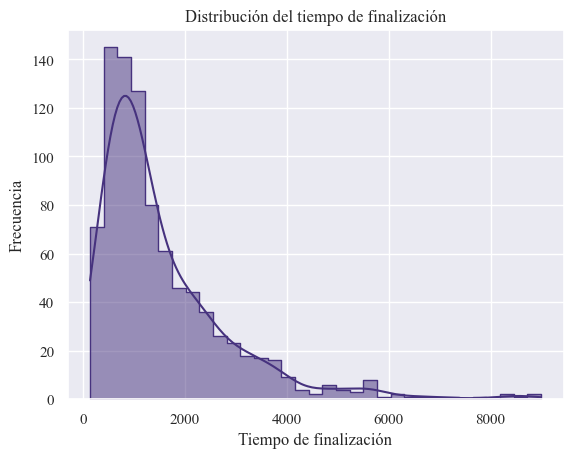
\includegraphics[height=.95\linewidth, width=.95\linewidth]{assets/time_dist}
			\caption{}
			\label{fig:1a}
		\end{subfigure}
		\begin{subfigure}{.45\linewidth}
			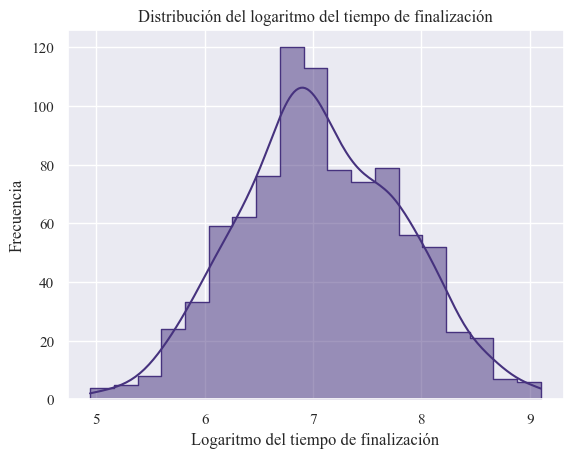
\includegraphics[height=.95\linewidth, width=.95\linewidth]{assets/log_time_dist}
			\caption{}
			\label{fig:1b}
		\end{subfigure}
		\caption{Histograma de la variable tiempo de finalización.}
		\label{fig:1}
	\end{figure}
	
	Para verificar la log-normalidad de la variable en cuestión, se muestra en la figura \ref{fig:2} una comparación entre los cuantiles muestrales, y teóricos de dicha distribución. La línea en el gráfico es evidencia de la similitud entre las dos métricas que se traduce en apoyo a la hipórtesis de normalidad del logaritmo de la variable. Para más certeza, se realiza una prueba de bondad de ajuste Kolmogorov-Smirnov que arroja un \emph{p-value} $ = 0.35$ confirmando lo anteriormente planteado.
	
	\begin{figure}[htb!]
		\centering
		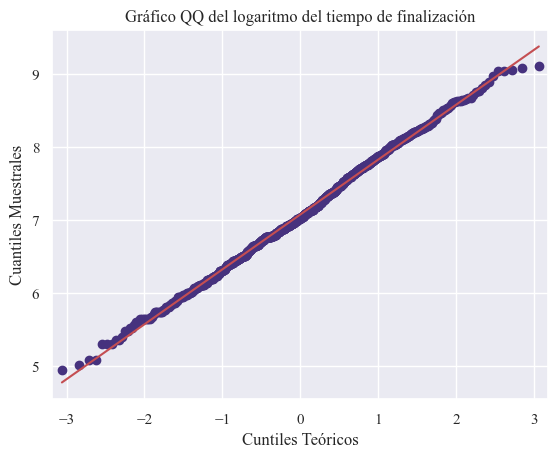
\includegraphics[height = .50\linewidth, width=.50\linewidth]{assets/log_time_qq}
		\caption{Gráfico Cuantil-Cuantil del logaritmo del  \emph{tiempo de finalización}.}
		\label{fig:2}
	\end{figure}
	
\subsection{Número de trabajadores y desempeño del equipo}

	No siempre cantidad significa calidad, y en terminos de desarrollo, mayor cantidad personas no necesariamente significa una menor tiempo de respuesta. Pero sí es cierto que, un mayor número de individuos se traduce a una mayor capacidad de ejecutar tareas en paralelo. En nuestras simulaciones existen dos variables que pueden describir estas dinámicas, el \emph{tiempo de finalización} y el \emph{número de trabajadores}, esta última fue contemplada en el rango de 2 a 10, para cada equipo.
	
	En la figura \ref{fig:3} se observa la relación entre las variables \emph{tiempo de finalización} y \emph{número de trabajadores}: los datos muestran una ligera tendencia del tiempo a decrecer, a medida que aumenta el tamaño del equipo. Esta observación es respaldada por un índice de correlación de $-0.59$ entre las dos variables.
	
	\begin{figure}[htb!]
	\centering
	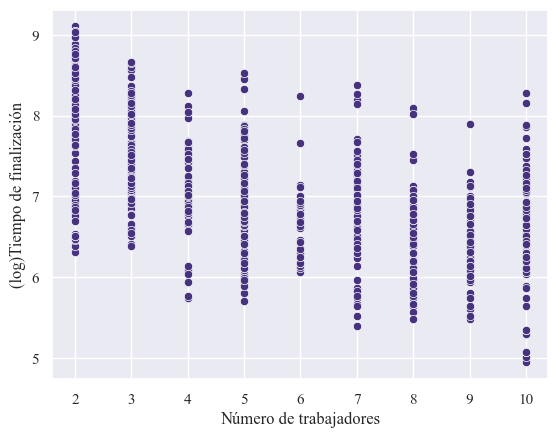
\includegraphics[height = .50\linewidth, width=.50\linewidth]{assets/log_time_wnumber_scatter}
	\caption{Gráfico de Dispersión (Scatterplot) del logaritmo del  \emph{tiempo de finalización} contra el \emph{número de trabajadores}.}
	\label{fig:3}
	\end{figure}
	
	Otro acercamiento para analizar la relación entre el tamaño del equipo y su desempeño puede observarse en la figura \ref{fig:4}. El \emph{número de trabajadores} fue dividido en dos categorías: equipos de hasta 5 (Grupo1), y equipos con más de 5 trabajadores (Grupo 2). Con esta nueva definición podemos ver como se comporta la distribución del (logaritmo) tiempo dentro de estos dos grupos. En la gráfica, ambas distribuciones parecen ser significativamente diferentes; lo cual es confirmado tras realizar una prueba T entre ambos grupos, fue definida como hipótesis alternativa: la media del Grupo 1 es mayor que la del Grupo 2, \emph{p-value} = 6.98e-55.
	
	\begin{figure}[htb!]
		\centering
		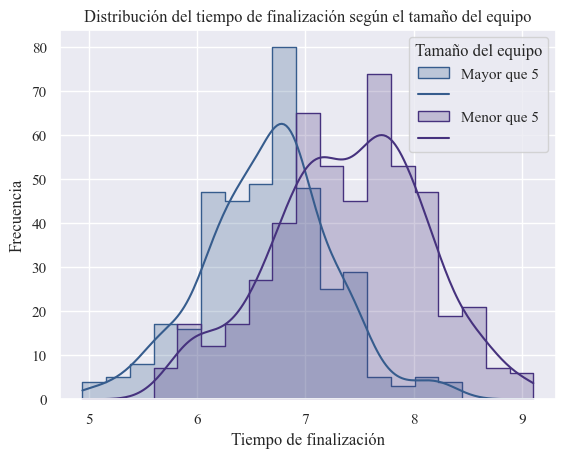
\includegraphics[height = .50\linewidth, width=.50\linewidth]{assets/log_time_wnumber_dist}
		\caption{Histograma del logaritmo del  \emph{tiempo de finalización} dentro de las categorías auxiliares del \emph{número de trabajadores}.}
		\label{fig:4}
	\end{figure}
	
\subsection{Audacia y oportunismo en el desempeño}
	Entre las características del Project Manager más interesantes que están presentes en la simulación, está la \emph{audacia} (\texttt{pm\_risky}) que da una idea de que tan propenso es a tomar decisiones arriesgadas en su obrar. Además se tiene en cuenta una métrica de la \emph{cantidad de decisiones arriesgadas} (u oportunidades, \texttt{pm\_take\_chance}) ha tomado a lo largo de la simulación. En la presente sección se analiza la influencia de estas variables en el desempeño, es decir en la optimización del tiempo.
	 
	 Se observa, en la figura \ref{fig:5}, la distribucion de la \emph{cantidad de decisiones arriesgadas} tomadas por el administrador, así como medidas: media y mediana. Estas medidas fueron tomadas para la creación de una variable categórica auxiliar que resuma la informacion de esta variable. De estra forma son constituidas las categorías: cantidad de decisiones mayor a la mediana (Grupo 1, en este contexto) y menores e igules (Grupo 2).

	\begin{figure}[htb!]
		\centering
		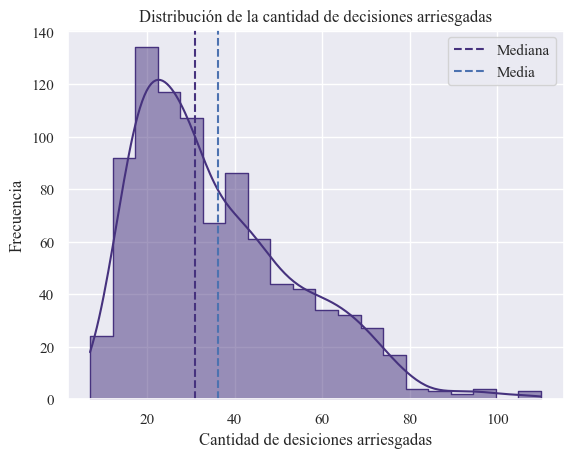
\includegraphics[height = .50\linewidth, width=.50\linewidth]{assets/take_chance_dist}
		\caption{Histograma del logaritmo del  \emph{tiempo de finalización} dentro de las categorías auxiliares del \emph{número de trabajadores}.}
		\label{fig:5}
	\end{figure}
	
	Con esta variable de apoyo de nuestro lado, podemos apreciar la compleja relación desempeño-audacia-riesgo en la figura \ref{fig:6}, que sugiere una correlación negativa entre audacia y desempeño, afectada por la cantidad de riesgos tomados (a mayor riesgo, menos negatividad de la relación).
	
	\begin{figure}[htb!]
		\centering
		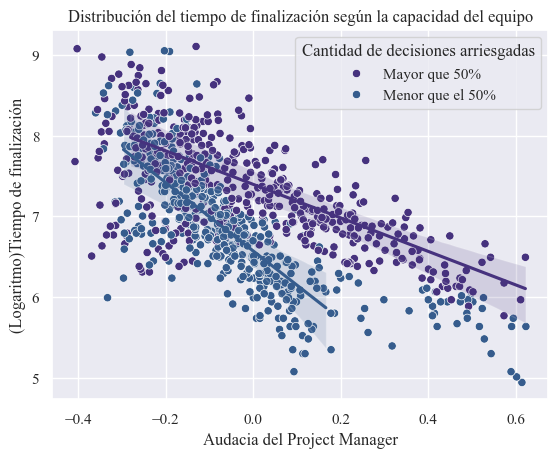
\includegraphics[height = .50\linewidth, width=.50\linewidth]{assets/risky_time_scatter}
		\caption{Gráfico de dispersion del logaritmo del  \emph{tiempo de finalización} y la \emph{audacia} del Project Manager, dentro de las categorías auxiliares de la \emph{cantidad de  decisiones arriesgadas} tomadas.}
		\label{fig:6}
	\end{figure}
	
	Para apoyar esta linea de pensamiento, se construyó un modelo de regresión lineal, con \texttt{pm\_risky} y \texttt{pm\_take\_chance} como variables independientes, y el logaritmo del tiempo como variable dependiente. Un fragmento de los resumen del modelo fue extraído y es presentado en la tabla de la figura \ref{table:1}. Nótese los signos de los coeficientes: como \texttt{pm\_risky} aporta negativamente al tiempo y \texttt{pm\_take\_chance} positivamente en menor medida, y ambas son variables significativas para describir el tiempo. 
	
	Se presenta además una visualización del ajuste del modelo de regresión lineal múltiple en la figura \ref{fig:7}.
	
	\begin{figure*}[ht!]%
		\begin{center}
			\begin{tabular}{lcccccc}
				\hline
				\multicolumn{1}{c}{\textbf{}} & \multicolumn{1}{c}{\textbf{coef}} & \multicolumn{1}{c}{\textbf{std err}} &\multicolumn{1}{c}{\textbf{t}} &\multicolumn{1}{c}{$\boldsymbol{ P>|t| }$} & \multicolumn{1}{c}{\textbf{[0.025 }} &\multicolumn{1}{c}{\textbf{0.975]}} \\		                                                
				\hline	  		
				const           		    &      6.3592    &   0.039 &   164.232&      0.000&       6.283 &      6.435  \\
				pm\_risky       			  &      -2.3674  &    0.085    &-28.000   &   0.000   &   -2.533    &  -2.201     \\
				pm\_take\_chance	 &     0.0182      &    0.001     &19.122    &  0.000    &   0.016     &  0.020      \\
				\hline
			\end{tabular}
			\caption{Fragmento del resumen de la regresión lineal múltiple.\label{table:1}}
		\end{center}
	\end{figure*}

	\begin{figure}[htb!]
	\centering
	\begin{subfigure}{.45\linewidth}
		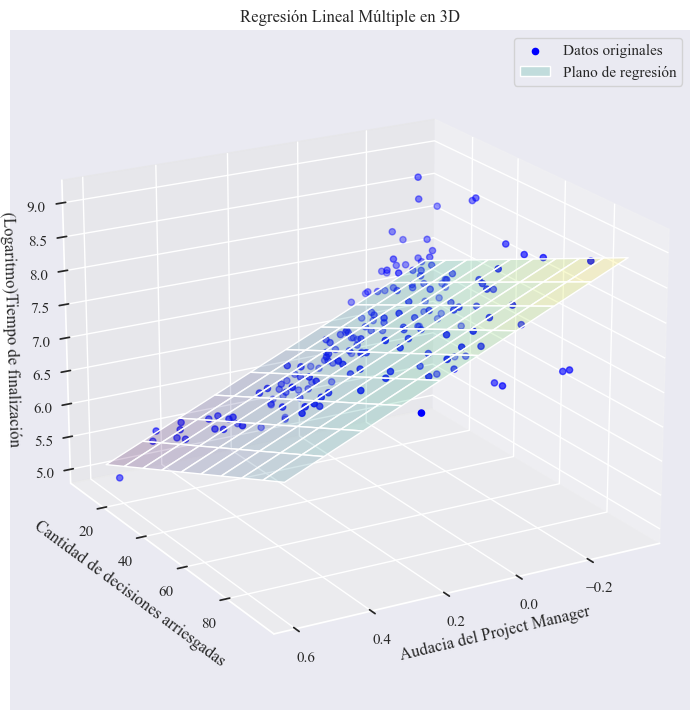
\includegraphics[height=.95\linewidth, width=.95\linewidth]{assets/multireg1}
		\caption{}
		\label{fig:7a}
	\end{subfigure}
	\begin{subfigure}{.45\linewidth}
		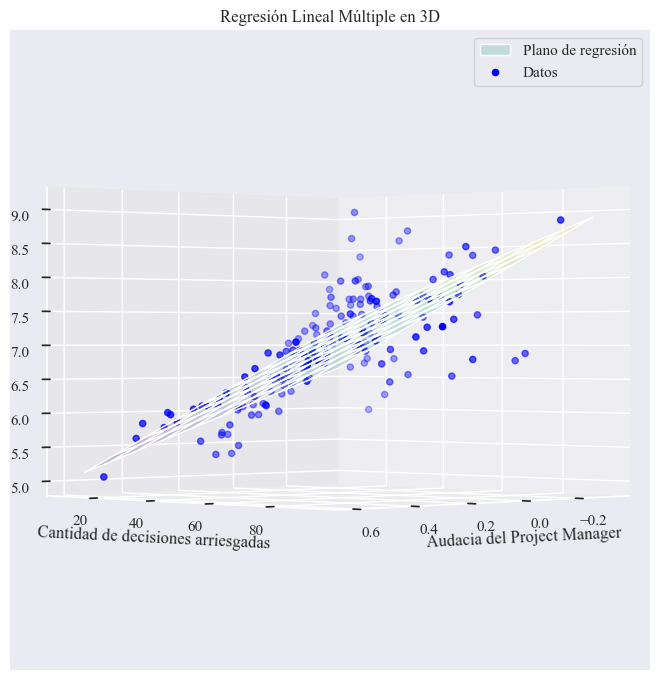
\includegraphics[height=.95\linewidth, width=.95\linewidth]{assets/multireg2}
		\caption{}
		\label{fig:7b}
	\end{subfigure}
	\caption{Gráfico de Dispersión y plano de ajuste de la regresión lineal.}
	\label{fig:7}
\end{figure}
\section{Conclusiones}
Una de las principales conclusiones es que el \emph{tiempo de finalización} de las tareas presenta un comportamiento log-normal, lo que fue corroborado tanto visualmente como mediante pruebas estadísticas, incluyendo la prueba de Kolmogorov-Smirnov, con un p-value de 0.35. Este hallazgo es crucial, ya que implica que el uso del logaritmo del tiempo de finalización puede ser un enfoque adecuado para analizar la distribución del desempeño de los equipos. Además, al observar esta distribución, queda claro que todos los equipos fueron capaces de completar las tareas dentro del tiempo disponible. Sin embargo, la capacidad de los equipos para minimizar el tiempo de ejecución dentro de esta ventana es un indicador significativo de su eficiencia. Este análisis refuerza la idea de que un desempeño superior se refleja en la capacidad de los equipos para reducir el tiempo de finalización de las tareas, independientemente de la holgura en la programación general del proyecto.

Por otro lado, se observó una relación inversa entre el número de trabajadores y el tiempo de finalización de las tareas. En la simulación, los equipos con más miembros mostraron una tendencia a completar las tareas en menos tiempo, lo que es coherente con la noción de que un mayor número de personas facilita la ejecución de tareas en paralelo. Esta correlación negativa (\(r = -0.59\)) indica una relación moderadamente fuerte, lo que sugiere que aumentar el número de trabajadores puede ser una estrategia efectiva para mejorar la eficiencia del equipo. No obstante, el análisis adicional revela matices interesantes: al dividir los equipos en dos grupos, aquellos con menos de 5 trabajadores y aquellos con más de 5, se encontró una diferencia significativa en los tiempos de finalización. El grupo de equipos más grandes fue consistentemente más eficiente, tal como lo demuestra la prueba T realizada, que arrojó un p-value extremadamente bajo (6.98e-55), lo que indica que la diferencia entre ambos grupos es estadísticamente significativa. Este resultado subraya que la cantidad de trabajadores puede tener un impacto notable en la capacidad del equipo para ejecutar tareas de manera eficiente, aunque el aumento del tamaño del equipo no garantiza necesariamente una mejora proporcional en la reducción del tiempo de finalización.

En cuanto al rol del \textbf{Project Manager}, se evidencian efectos complejos en su influencia sobre el desempeño del equipo. En particular, la \emph{audacia} del Project Manager, medida a través de la variable "\texttt{pm risky}", mostró tener un impacto negativo en el tiempo de finalización de las tareas, lo que sugiere que una actitud demasiado arriesgada puede aumentar la capacidad del equipo para completar las tareas de manera eficiente (al disminuir el tiempo de finalización). No obstante, este efecto negativo no es tan simple como parece. El número de decisiones arriesgadas tomadas (\texttt{pm\_take\_chance}) actúa como un moderador que mitiga la relación negativa entre la audacia y el desempeño. Es decir, los Project Managers que toman decisiones arriesgadas de manera calculada logran aumenta el impacto negativo que tendría la audacia por sí sola. A medida que se incrementa la cantidad de riesgos tomados, el efecto de la audacia sobre el tiempo de finalización disminuye (haciendo que empeore el tiempo), lo que implica que la capacidad de un Project Manager para gestionar el riesgo de manera eficiente puede mejorar el desempeño del equipo. Este hallazgo es apoyado por el modelo de regresión lineal, que revela que ambas variables (\texttt{pm\_risky} y \texttt{pm\_take\_chance}) son significativamente importantes para explicar el tiempo de finalización. Específicamente, los coeficientes del modelo indican que mientras la audacia afecta negativamente al tiempo de finalización, la cantidad de riesgos tomados tiene un efecto positivo, aunque en menor magnitud. Esto indica que un Project Manager audaz pero que toma riesgos de manera bien calculada puede mejorar el desempeño del equipo.

En conjunto, los hallazgos sugieren que la eficiencia de los equipos no solo depende del número de trabajadores, sino también de la estrategia de liderazgo del Project Manager. Un liderazgo que combina audacia con una toma de riesgos calculada puede ser clave para optimizar el tiempo de finalización de las tareas. Al mismo tiempo, aumentar el tamaño del equipo parece mejorar el desempeño en términos de reducción del tiempo, aunque esto debe considerarse con cuidado, ya que un aumento excesivo en el número de trabajadores no necesariamente garantiza una mejora proporcional.

La simulación multiagente con la arquitectura BDI nos permitió modelar un entorno de trabajo colaborativo donde los agentes toman decisiones complejas de manera autónoma. El uso de un algoritmo genético para la optimización de tareas, junto con la lógica difusa para la evaluación de las situaciones, resultó en una mayor flexibilidad y adaptabilidad del sistema. La incorporación de aprendizaje reforzado mejoró las capacidades del \textbf{Project Manager}, haciéndolo más eficiente en la gestión de proyectos y la optimización del uso de los recursos a largos plazos.

\end{document}
